\documentclass[a4paper,12pt]{ctexart}

\usepackage{geometry}
\usepackage{booktabs}
\usepackage{graphicx}
\usepackage[final]{pdfpages}
\usepackage[stable]{footmisc}
\usepackage{threeparttable}
\usepackage{indentfirst}
\usepackage{minted}
\usepackage{listings}
\usepackage{xcolor}
\usepackage{subfigure}
\usepackage{amsmath}
\usepackage{amsfonts}

% \setlength{\parindent}{0pt}
\geometry{top=20mm,bottom=20mm,left=20mm,right=20mm}
\lstset{
    rulesepcolor= \color{gray},
    breaklines=true,
    numbers=left,
    numberstyle= \small,
    commentstyle=\color{gray},
    frame=shadowbox
}

\title{Y23T2W5 例行周报}
\author{杜睿}
% \date{}

\begin{document}
% \tableofcontents
\maketitle

% \begin{abstract}
% \end{abstract}

为了争取复现上周毛振洋学长报告的\cite{10228982}Transformer,我这周主要进行了两次深度学习实验,熟悉了深度学习框架及其实现。

\section{基础之回归:新冠人数预测}

这个问题是输入前两天的相关信息(地区、问卷)和确诊人数,第三天的相关信息(地区、问卷等),输出第三天的新冠确诊人数。

首先,特征选择非常重要。某些和结果关联性不大甚至是毫无关系的属性越多,越是一种负担;在训练数据少的情况下,机器学习算法可能无法提取正确的模式和规律,因此需要人工介入对原始数据进行变换。本次数据不存在数据缺失,因此主要是选择合适的特征,对量纲不一致的特征每列进行标准化。

\begin{figure}[htbp]
    \centering
    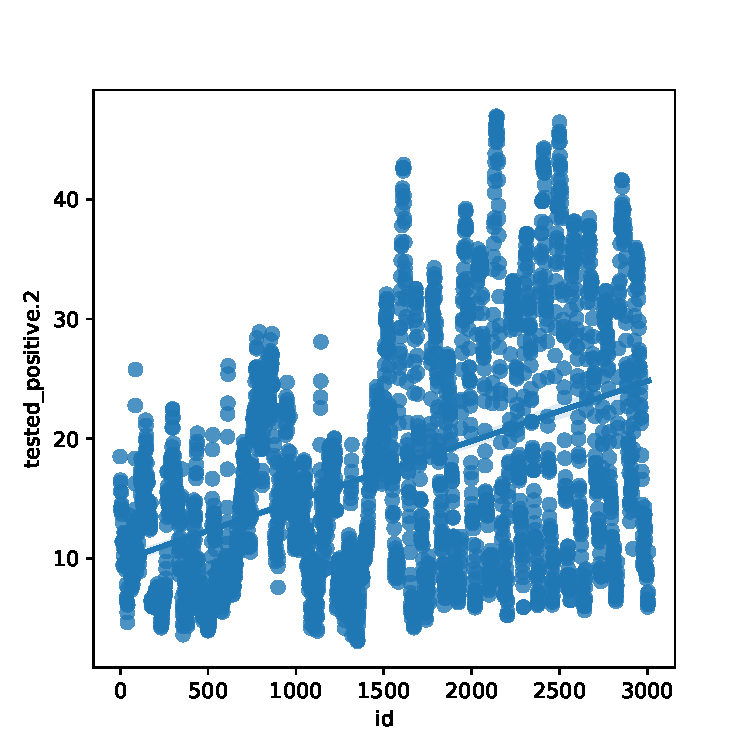
\includegraphics[width=0.45\linewidth]{1.pdf}
    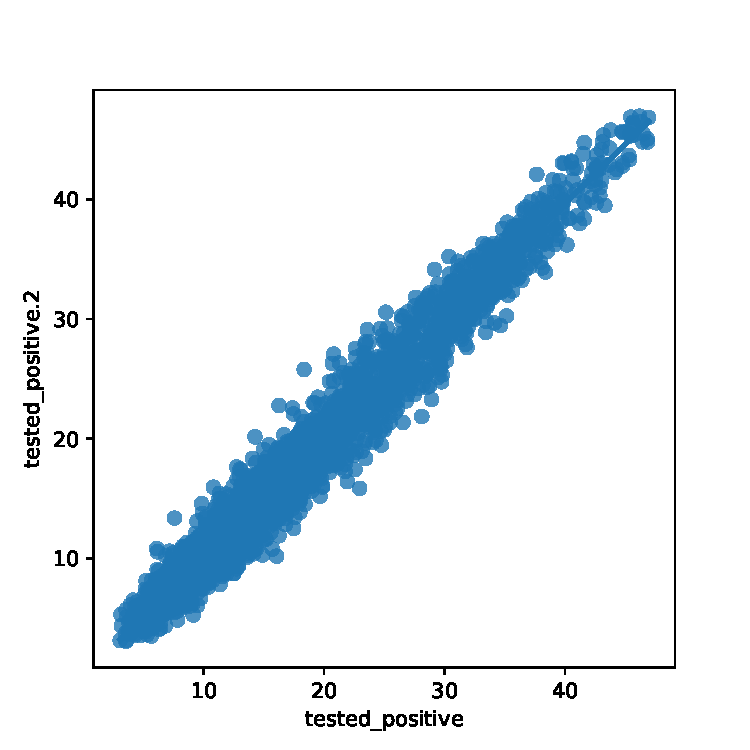
\includegraphics[width=0.45\linewidth]{0.pdf}
    \caption{ID(左)与前日确诊人数(右)与当日确诊人数}
\end{figure}

其次,需要标定合适的模型。训练资料只有3009笔,因此模型如果过于复杂,不仅可能导致过拟合,还可能导致后续优化困难。本次我采用基于残差块的简易多层神经网络,没有使用BatchNorm或SyncBatchNorm。跳层连接的实现如下:

\begin{lstlisting}[language={python},caption={模型实现}]
class ResBlock(nn.Module):
    def __init__(self, hidden_size):
        super(ResBlock, self).__init__()
        self.fc1 = nn.Linear(hidden_size, hidden_size)
        self.fc2 = nn.Linear(hidden_size, hidden_size)
        self.act = nn.ReLU6()

    def forward(self, x):
        return self.act(x + self.fc2(self.act(self.fc1(x))))


class My_Model(nn.Module):
    def __init__(self, input_size, hidden_size=64, output_size=1, depth=5):
        super(My_Model, self).__init__()

        # TODO: modify model's structure, be aware of dimensions.
        layers = nn.ModuleList()
        layers.extend([nn.Linear(input_size, hidden_size), nn.ReLU()])
        layers.extend([ResBlock(hidden_size) for _ in range(depth)])
        layers.append(nn.Linear(hidden_size, output_size))
        self.layers = nn.Sequential(*layers)

    def forward(self, x):
        return self.layers(x).squeeze(1)  # (B, 1) -> (B)

\end{lstlisting}

实验过程中,在残差块堆叠层数和学习率设置变化时,损失可能会为NaN,因此这里使用ReLU6作为激活函数。

最后,要考虑如何求解最优化问题。我们假定损失函数为MSE Loss;优化算法的选择不同,获得结果的质量和迭代时间也不同。

此外,还有许多超参数需要人为事先定义,例如,学习率、残差块层数、预热轮数等等。为了选择合适的超参数,我采用Weights Bias库对超参数的可行方案进行贝叶斯优化,以寻找最佳的超参数。由于测试集无从得知,因此,我们要么以采用留出法按一定的比例划分训练集和开发集,或者采用交叉验证的方式对超参数进行评价。

实验采用5折交叉验证,重复2次的方式,进行了实验,采用交叉验证损失最低的超参数重新进行训练,并采用K折Bagging的方式将10个模型的输出结果进行平均。

\begin{figure}[htbp]
    \centering
    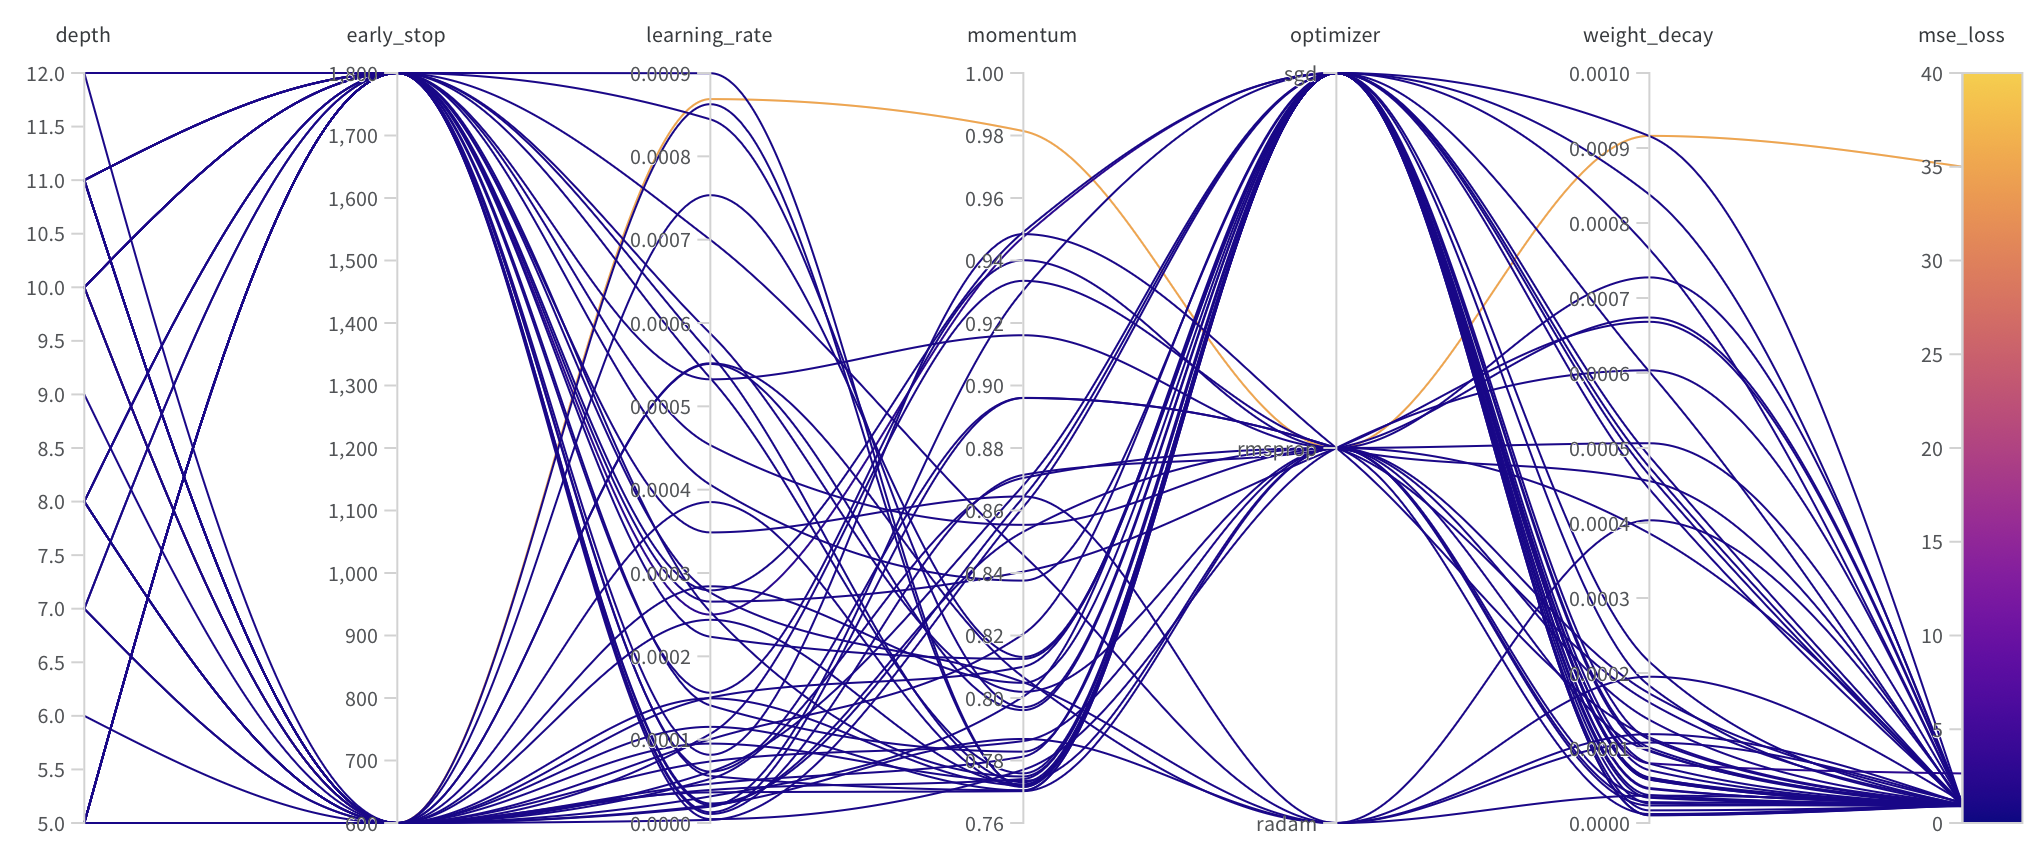
\includegraphics[width=0.8\linewidth]{WB.png}
    \caption{超参数搜索}
\end{figure}

最后,在交叉验证中损失为0.7612,但是在Kaggle Private Leaderboard上损失为0.93204。这个结果让我比较意外,因为从理论上说交叉验证可以有效地防止在训练集上过拟合,丧失泛化能力,而交叉验证又避免了由于划分不均匀导致的偏差。虽然本次实验采用了深度神经网络,但实际上这个问题的数据规模远不及如今大数据时代,因此,我在考虑是否要添加Dropout、减少模型参数与复杂度,人工对特征进行选择。

本次实验不仅训练了Pytorch深度学习框架与流程,还尝试了各种优化器、动态学习率调整策略、wandb与tensorboard日志,模型参数的初始化、k-折交叉验证。

\section{基础之分类:语音音标分类}

这个问题是输入一个语音,即输入(T, 39)的张量,对于每一帧而言标注音标,输出(T)的张量。这个问题的特殊性在于,一语音帧(大约一秒)的音标具有时间序列的属性,可能因为前后音标具有关联性。

因此,一种朴素的想法是,人工进行数据处理,将一帧与其前后k帧进行连接,然后作为模型输入,输出一个类别;这样,便以人工的形式考虑了上下文信息,而且规避了每条语音长短不一导致输入维度不一致的问题。此外,有一类模型专门负责处理序列输入与序列输出的问题,即RNN。

对于朴素的想法的实现以及验证而言,无需训练特别长的时间准确率便可以达到0.49735(Kaggle)。

对于采用RNN的方式,目前结果和我预测差距非常大。我实现了自定义Dataset加载数据,基于GRU的模型Tagger,实现了collate\_fn用于将长度不一的语音补零后组织成批次,基于交叉熵实现了criterion用于将长短不一批次的输出序列和Ground Truth进行比较计算损失。但是,无论我怎么调整层数、学习率等参数,损失始终降不下去,准确率始终不高于0.2。

\begin{figure}[htbp]
    \centering
    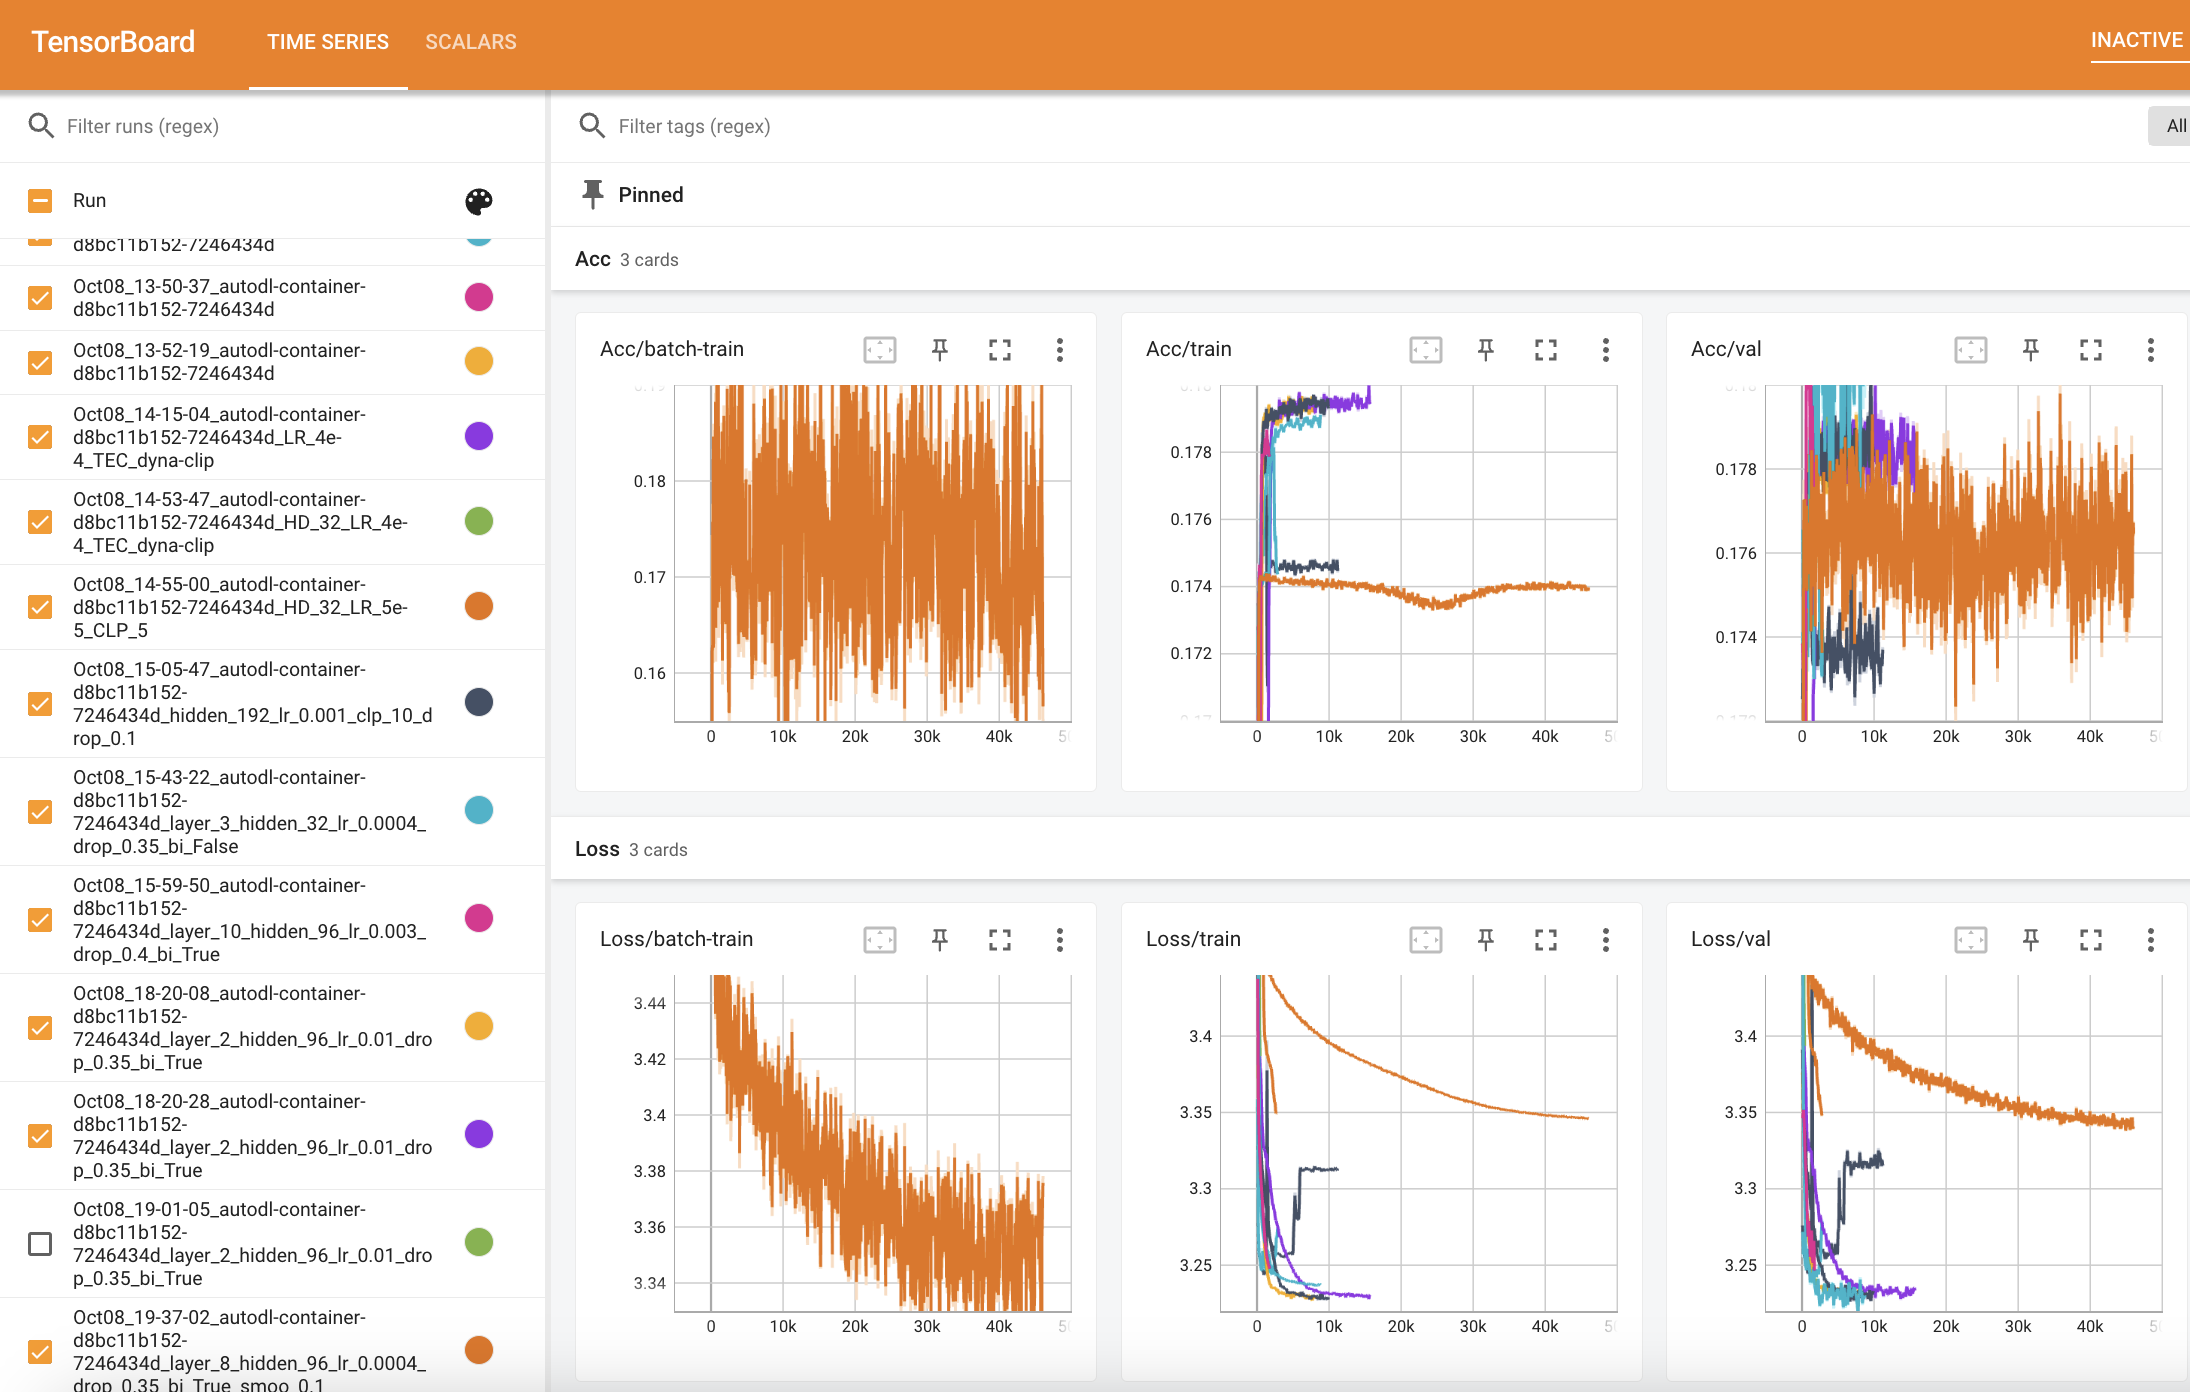
\includegraphics[width=0.9\linewidth]{TB.png}
    \caption{训练日志}
\end{figure}

网上说的,要调小学习率:没用。

网上说的,要梯度裁剪:也没用。

\section{总结}
理论和现实,思考和实操总是存在差距。还是要动手做,才能发现问题。下周一个重要的任务,就是修改RNN的代码,让它发挥理论上应该有的作用。

\bibliography{main}
\bibliographystyle{ieeetr}

\end{document}

% \begin{table}[htbp]
%     \caption{常用的处理机调度策略}
%     \centering

%     \begin{threeparttable}
%         \begin{tabular}{cccccc}
%             \toprule
%             算法名称           & 主要适用范围       & 默认调度方式         \\
%             \midrule
%             先来先服务         & 作业调度\&进程调度 & 非抢占式             \\
%             短作业(进程)优先 & 作业调度\&进程调度 & 非抢占式             \\
%             高响应比优先       & 作业调度           & 非抢占式             \\
%             时间片轮转         & 进程调度           & 抢占式(不抢时间片) \\
%             多级反馈队列       & 进程调度           & 抢占式(抢占时间片) \\
%             \bottomrule
%         \end{tabular}

%         \zihao{-6}
%         \begin{tablenotes}
%             \item [*]   调度策略也就是调度算法
%         \end{tablenotes}

%     \end{threeparttable}
%     \qquad
% \end{table}

% \begin{figure}[htbp]
%     \centering
%     \includegraphics[height=550pt]{v1-class-compat.png}
%     \caption{UML类图(第二版)}
% \end{figure}

% \begin{minted}[mathescape,
%     linenos,
%     numbersep=5pt,
%     frame=lines,
%     gobble=4,
%     framesep=2mm]{Java}
%     public interface Observable {
%         void attachObserver(Observer o);

%         void detachObserver(Observer o);

%         void notifyObservers();
%     }
% \end{minted}

% \begin{lstlisting}[language={java},caption={收容队列(基于响应比的优先队列)}]
% private PriorityQueue<Task> queue = new PriorityQueue<>(new Comparator<Task>() {
%     @Override
%     public int compare(Task o1, Task o2) {
%         return (o2.getResponseRate(Clock.minutes) - o1.getResponseRate(Clock.minutes) > 0) ? (1) : (-1);
%     }
% });
% \end{lstlisting}